\section{WebGL}

\subsection{Pipeline}
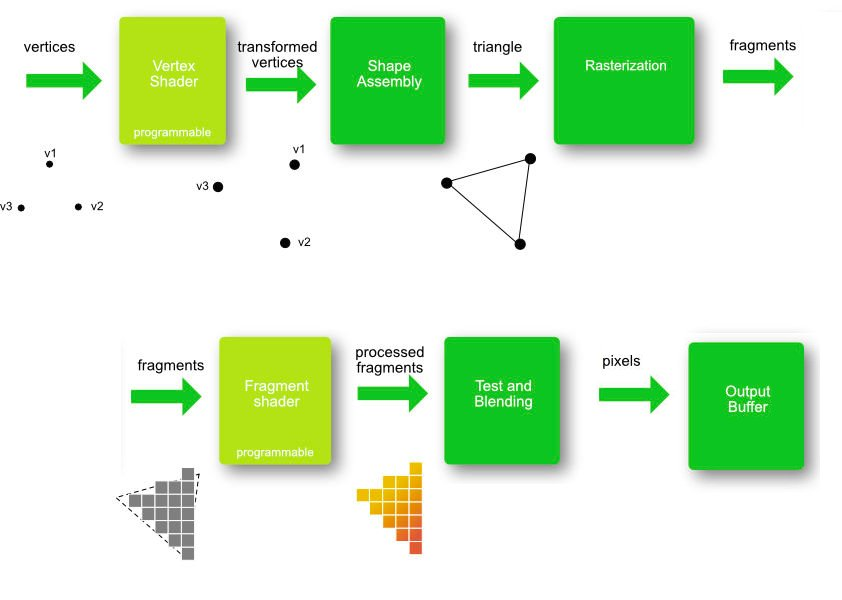
\includegraphics[width=0.9\textwidth]{images/graphicPipeline.jpg}

\subsection{Engine}

\begin{lstlisting}{webgl.ts}
    /**
    * WEBGL
    *
    * Allows to draw points, line segments, or triangles.
    *
    * Vertex shaders take whatever coordinates you use and return a 3-d array with elements between -1 and 1.
    * Basically, this is a 3d-array, but WebGl does not use the z-axis for real perspective, but only to differentiate
    * what pixel lies in front of another.
    * This is not like looking in a 3d-box, but rather like looking on multiple stacked sheets on a projector.
    *
    * WebGL knows two data structures:
    *  - buffers (generic byte arrays): usually positions, normals, texture-coordinates, vertex-colors etc.
    *    buffers are accessed in shaders as 'attributes'.
    *    note that buffers contain one entry for each vertex.
    *  - textures (bitmap images).
    *
    * Shaders use these data structures in two different ways.
    *  - Attributes are values, one per vertex.
    *    For the shader, attributes are read-only.
    *    Attributes default to [0, 0, 0, 1]
    *  - Uniforms are values, one per shader.
    *    For the shader, uniforms are read-only.
    *
    * Apart from this, shaders know about two more types of data:
    *  - Varyings are values that are passed from vertex-shader to fragment-shader.
    *    They are read-only only for the fragment-shader.
    *  - Const: a compile-time constant.
    *
    * A program is just a list of compiled and linked vertex- and fragment-shaders.
    *
    *
    * Drawing: there's drawArrays and drawElements.
    *  - drawArrays is the robust all-rounder.
    *  - drawElements can be more performant if you share vertices between objects.
    *
    *
    * Rendering data is fast, but uploading it into GPU memory is slow.
    * Optimizing WebGl performance mostly means: Avoiding having GPU and CPU wait for each other.
    * The more the GPU can do in bulk, the better. The more often you have to upload data from CPU to GPU, the worse.
    *  - So avoid switching programs, buffers and uniforms if you can.
    *    (You won't be able to avoid switching buffers, because every object is likely different. But sort your objects by their shaders, and you'll save a lot of time.)
    *  - Try to do translations, rotations and shears inside the vertex-shader instead of altering the object's buffer.
    *  - If appropriate, create über-shaders and über-buffers, that contain information for more than just one object.
    *
    * There is another thing that affects performance:
    * WebGL will only run fragment-shaders when the object's pixels aren't already obscured by a larger object in front of it.
    * That means it makes sense to first draw large objects that are close to the camera - all objects behind them won't need their fragment-shader executed.
    */
   
   
   
   
   /**
    * Compile shader.
    */
   const compileShader = (gl: WebGLRenderingContext, typeBit: number, shaderSource: string): WebGLShader => {
       const shader = gl.createShader(typeBit);
       gl.shaderSource(shader, shaderSource);
       gl.compileShader(shader);
       if (!gl.getShaderParameter(shader, gl.COMPILE_STATUS)) {
           gl.deleteShader(shader);
           throw new Error('An error occurred compiling the shader: ' + gl.getShaderInfoLog(shader));
       }
       return shader;
   };
   
   
   /**
    * Note that every program *must* have one and only one vertex-shader
    * and one and only one fragment shader.
    * That means you cannot add multiple fragment-shaders in one program. Instead, either load them in consecutively as part of different programs,
    * or generate an über-shader that contains both codes.
    */
   export const initShaderProgram = (gl: WebGLRenderingContext, vertexShaderSource: string, fragmentShaderSource: string): WebGLProgram => {
   
       const program = gl.createProgram();
   
       const vertexShader = compileShader(gl, gl.VERTEX_SHADER, vertexShaderSource);
       const fragmentShader = compileShader(gl, gl.FRAGMENT_SHADER, fragmentShaderSource);
       gl.attachShader(program, vertexShader);
       gl.attachShader(program, fragmentShader);
   
       gl.linkProgram(program);
   
       if (!gl.getProgramParameter(program, gl.LINK_STATUS)) {
           gl.deleteProgram(program);
           throw new Error('Unable to initialize the shader program: ' + gl.getProgramInfoLog(program));
       }
   
       return program;
   };
   
   
   export const setup3dScene = (gl: WebGLRenderingContext): void => {
       gl.viewport(0, 0, gl.canvas.width, gl.canvas.height);
   
       gl.enable(gl.DEPTH_TEST);
       gl.depthFunc(gl.LEQUAL);
       gl.cullFace(gl.BACK);
   
       clearBackground(gl, [0, 0, 0, 1]);
   };
   
   
   export const bindProgram = (gl: WebGLRenderingContext, program: WebGLProgram): void => {
       gl.useProgram(program);
   };
   
   
   export const clearBackground = (gl: WebGLRenderingContext, color: number[]): void => {
       gl.clearColor(color[0], color[1], color[2], color[3]);
       gl.clearDepth(1.0);
       gl.clear(gl.COLOR_BUFFER_BIT | gl.DEPTH_BUFFER_BIT);
   };
   
   
    /**
     * A generic buffer, together with it's metadata.
     */
   export interface BufferObject {
       buffer: WebGLBuffer;
       vectorSize: number;
       vectorCount: number;
       type: number;
       normalize: boolean;
       stride: number;
       offset: number;
   }
   
   
   /**
    * Create buffer. Creation is slow! Do *before* render loop.
    */
   export const createFloatBuffer = (gl: WebGLRenderingContext, data: number[][]): BufferObject => {
   
       const dataFlattened = new Float32Array([].concat.apply([], data));
   
       const buffer = gl.createBuffer();
       gl.bindBuffer(gl.ARRAY_BUFFER, buffer);
       gl.bufferData(gl.ARRAY_BUFFER, dataFlattened, gl.STATIC_DRAW);
       // STATIC_DRAW: tells WebGl that we are not likely to change this data much.
   
       const bufferObject: BufferObject = {
           buffer: buffer,
           vectorSize: data[0].length,
           vectorCount: data.length,
           type: gl.FLOAT,   // the data is 32bit floats
           normalize: false, // don't normalize the data
           stride: 0,        // 0 = move forward size * sizeof(type) each iteration to get the next position. Only change this in very-high-performance jobs.
           offset: 0,        // start at the beginning of the buffer. Only change this in very-high-performance jobs.
       };
   
       return bufferObject;
   };
   
   
   
   export const createTexture = (gl: WebGLRenderingContext, image: HTMLImageElement): WebGLTexture => {
       const texture = gl.createTexture();
       gl.bindTexture(gl.TEXTURE_2D, texture);
       gl.texImage2D(gl.TEXTURE_2D, 0, gl.RGBA, gl.RGBA, gl.UNSIGNED_BYTE, image);
       gl.generateMipmap(gl.TEXTURE_2D); // mipmaps are mini-versions of the texture.
       return texture;
   };
   
   
   /**
    * Even though we reference textures as uniforms in a fragment shader, assigning an actual texture-value to that uniform works differently than for normal uniforms.
    * Normal uniforms have a concrete value.
    * Texture uniforms, on the other hand, are just an integer-index that points to a special slot in the GPU memory (the bindPoint) where the actual texture value lies.
    */
   export const bindTextureToUniform = (gl: WebGLRenderingContext, texture: WebGLTexture, bindPoint: number, uniformLocation: WebGLUniformLocation): void =>  {
       if (bindPoint > gl.getParameter(gl.MAX_COMBINED_TEXTURE_IMAGE_UNITS)) {
           throw new Error(`There are only ${gl.getParameter(gl.MAX_COMBINED_TEXTURE_IMAGE_UNITS)} texture bind points, but you tried to bind to point nr. ${bindPoint}.`);
       }
       gl.activeTexture(gl.TEXTURE0 + bindPoint);  // analog to enableVertexAttribArray
       gl.bindTexture(gl.TEXTURE_2D, texture);  // analog to bindBuffer
       gl.uniform1i(uniformLocation, bindPoint); // analog to vertexAttribPointer
   };
   
   
   /**
    * Fetch attribute's location (attribute declared in some shader). Slow! Do *before* render loop.
    */
   export const getAttributeLocation = (gl: WebGLRenderingContext, program: WebGLProgram, attributeName: string): number => {
       const loc = gl.getAttribLocation(program, attributeName);
       if (loc === -1) {
           throw new Error(`Couldn't find attribute ${attributeName} in program.`);
       }
       return loc;
   };
   
   /**
    * Fetch uniform's location (uniform declared in some shader). Slow! Do *before* render loop.
    */
   export const getUniformLocation = (gl: WebGLRenderingContext, program: WebGLProgram, uniformName: string): WebGLUniformLocation => {
       const loc = gl.getUniformLocation(program, uniformName);
       if (loc === null) {
           throw new Error(`Couldn't find uniform ${uniformName} in program.`);
       }
       return loc;
   };
   
   
   /**
    * Attributes vary from vertex to vertex - that means that there are *many* of them.
    * So it makes sense for WebGl to store attribute values in a dedicated data structure - the buffer.
    */
   export const bindBufferToAttribute = (gl: WebGLRenderingContext, attributeLocation: number, bufferObject: BufferObject): void => {
       // Enable editing
       gl.enableVertexAttribArray(attributeLocation);
       // Bind buffer to ARRAY_BUFFER
       gl.bindBuffer(gl.ARRAY_BUFFER, bufferObject.buffer);
       // Bind the buffer currently at ARRAY_BUFFER to a vertex-buffer-location.
       gl.vertexAttribPointer(
           attributeLocation,
           bufferObject.vectorSize, bufferObject.type, bufferObject.normalize, bufferObject.stride, bufferObject.offset);
   };
   
   
   export type UniformType = '1i' | '2i' | '3i' | '4i' | '1f' | '2f' | '3f' | '4f';
   
   /**
    * Contrary to attributes, uniforms don't need to be stored in a buffer.
    */
   export const bindValueToUniform = (gl: WebGLRenderingContext, uniformLocation: WebGLUniformLocation, type: UniformType, values: number[]): void => {
       switch (type) {
           case '1i':
               gl.uniform1i(uniformLocation, values[0]);
               break;
   
           case '1f':
               gl.uniform1f(uniformLocation, values[0]);
               break;
           case '2f':
               gl.uniform2f(uniformLocation, values[0], values[1]);
               break;
           case '3f':
               gl.uniform3f(uniformLocation, values[0], values[1], values[2]);
               break;
           case '4f':
               gl.uniform4f(uniformLocation, values[0], values[1], values[2], values[3]);
               break;
   
           default:
               throw Error(`Type ${type} not yet implemented.`);
       }
   };
\end{lstlisting}

\begin{lstlisting}{engine.core.ts}
    import { initShaderProgram, setup3dScene, createFloatBuffer, getAttributeLocation, bindBufferToAttribute, getUniformLocation, bindValueToUniform, clearBackground, BufferObject, UniformType, bindProgram, createTexture, bindTextureToUniform } from './webgl';
    const hash = require('string-hash');
    
    
    export interface IProgram {
        program: WebGLProgram;
        id: string;
    }
    
    
    export class Program implements IProgram {
    
        readonly program: WebGLProgram;
        readonly id: string;
    
        constructor(gl: WebGLRenderingContext, vertexShaderSource: string, fragmentShaderSource: string) {
            this.program = initShaderProgram(gl, vertexShaderSource, fragmentShaderSource);
            this.id = hash(vertexShaderSource + fragmentShaderSource);
        }
    }
    
    
    export interface IUniform {
        location: WebGLUniformLocation;
        type: UniformType;
        value: number[];
    }
    
    
    export class Uniform implements IUniform {
    
        readonly location: WebGLUniformLocation;
        readonly type: UniformType;
        readonly value: number[];
    
        constructor(gl: WebGLRenderingContext, program: IProgram, variableName: string, type: UniformType, data: number[]) {
            this.location = getUniformLocation(gl, program.program, variableName);
            this.type = type;
            this.value = data;
        }
    }
    
    
    export interface ITexture {
        location: WebGLUniformLocation;
        bindPoint: number;
        texture: WebGLTexture;
    }
    
    export class Texture implements ITexture {
    
        readonly location: WebGLUniformLocation;
        readonly bindPoint: number;
        readonly texture: WebGLTexture;
    
        constructor(gl: WebGLRenderingContext, program: IProgram, variableName: string, image: HTMLImageElement, bindPoint: number) {
            this.location = getUniformLocation(gl, program.program, variableName);
            this.texture = createTexture(gl, image);
            this.bindPoint = bindPoint;
        }
    }
    
    
    export interface IAttribute {
        location: number;
        value: BufferObject;
    }
    
    
    export class Attribute implements IAttribute {
    
        readonly location: number;
        readonly value: BufferObject;
    
        constructor(gl: WebGLRenderingContext, program: IProgram, variableName: string, data: number[][]) {
            this.location = getAttributeLocation(gl, program.program, variableName);
            this.value = createFloatBuffer(gl, data);
        }
    }
    
    
    interface IEntity {
        program: IProgram;
        attributes: IAttribute[]; // note that attributes must all have the same number of entries!
        uniforms: IUniform[];
        textures: ITexture[];
        update: (tDelta: number) => void;
    }
    
    
    
    export class Entity implements IEntity {
    
        constructor(
            readonly program: IProgram,
            readonly attributes: IAttribute[],
            readonly uniforms: IUniform[],
            readonly textures: ITexture[],
            readonly updateFunction: (tDelta: number, attrs: IAttribute[], unis: IUniform[]) => void) {}
    
        update(tDelta: number): void {
            this.updateFunction(tDelta, this.attributes, this.uniforms);
        }
    }
    
    
    
    
    export class Engine {
    
        readonly entities: IEntity[] = [];
    
        constructor() {}
    
        public renderLoop(gl: WebGLRenderingContext, fps: number): void {
            setup3dScene(gl);
    
            const tDeltaTarget = 1000 * 1.0 / fps;
            let tStart, tNow: number, tDelta: number, tSleep;
            let currentShader = '';
            const render = () => {
                tStart = window.performance.now();
    
                // Part 1: allow objects to update their state
                for (const e of this.entities) {
                    e.update(tDeltaTarget);
                }
    
                // Part 2: do the actual rendering work here
                clearBackground(gl, [.7, .7, .7, 1]);
                for (const e of this.entities) {
                    if (e.program.id !== currentShader) {
                        bindProgram(gl, e.program.program);
                        currentShader = e.program.id;
                    }
                    for (const a of e.attributes) {
                        bindBufferToAttribute(gl, a.location, a.value);
                    }
                    for (const u of e.uniforms) {
                        bindValueToUniform(gl, u.location, u.type, u.value);
                    }
                    for (const t of e.textures) {
                        bindTextureToUniform(gl, t.texture, t.bindPoint, t.location);
                    }
                    gl.drawArrays(gl.TRIANGLES, 0, e.attributes[0].value.vectorCount);
                }
    
                // Part 3: time-management
                tNow = window.performance.now();
                tDelta = tNow - tStart;
                tSleep = Math.max(tDeltaTarget - tDelta, 0);
                setTimeout(() => {
                    requestAnimationFrame(render);
                }, tSleep);
    
            };
    
            render();
        }
    
        public addEntity(entity: IEntity): void {
            this.entities.push(entity);
            this.sortEntities();
        }
    
    
        private sortEntities(): void {
            this.entities.sort((a: IEntity, b: IEntity) => {
                return (a.program.id > b.program.id) ? 1 : -1;
            });
        }
    
    
    }
\end{lstlisting}

\begin{lstlisting}{main.ts}
    import { Engine, Program, Entity, Attribute, Uniform, IAttribute, IUniform, Texture } from './engine/engine.core';
    import { box, square } from './engine/engine.shapes';
    const basic3dVertexShaderSource = require('./engine/shaders/basic3d.vert.glsl').default;
    const basic3dFragmentShaderSource = require('./engine/shaders/basic3d.frag.glsl').default;
    
    
    const canvas = document.getElementById('webGlCanvas') as HTMLCanvasElement;
    const gl = canvas.getContext('webgl');
    
    const letterImg = document.getElementById('letterTexture') as HTMLImageElement;
    const boxImg = document.getElementById('boxTexture') as HTMLImageElement;
    
    const engine = new Engine();
    
    const program = new Program(gl, basic3dVertexShaderSource, basic3dFragmentShaderSource);
    
    const letterEntity = new Entity(
        program,
        [
            new Attribute(gl, program, 'a_vertex', square(.2, .2) ),
            new Attribute(gl, program, 'a_textureCoord', square(.2, .2))
        ], [
            new Uniform(gl, program, 'u_translation', '3f', [.3, .3, .0]),
            new Uniform(gl, program, 'u_rotation', '3f', [.0, .0, .0])
        ], [
            new Texture(gl, program, 'u_texture', letterImg, 0)
        ],
        (tDelta: number, attrs: IAttribute[], unis: IUniform[]) => {
            unis[1].value[0] += 0.001 * tDelta;
            unis[1].value[1] += 0.001 * tDelta;
        });
    
    
    
    
    const boxEntity = new Entity(
        program,
        [
            new Attribute(gl, program, 'a_vertex', box(.2, .1, .3)),
            new Attribute(gl, program, 'a_textureCoord', box(.2, .1, .3))
        ], [
            new Uniform(gl, program, 'u_translation', '3f', [-.3, -.3, -.3]),
            new Uniform(gl, program, 'u_rotation', '3f', [.0, .0, .0])
        ], [
            new Texture(gl, program, 'u_texture', boxImg, 1)
        ],
        (tDelta: number, attrs: IAttribute[], unis: IUniform[]) => {
            unis[1].value[0] += 0.001 * tDelta;
            unis[1].value[1] += 0.001 * tDelta;
        }
    );
    
    
    
    engine.addEntity(letterEntity);
    engine.addEntity(boxEntity);
    
    engine.renderLoop(gl, 30);
    
\end{lstlisting}

\subsection{Shader gallery}


